\documentclass[12pt]{article}

\usepackage{sbc-template}
\usepackage{graphicx,url}
\usepackage[utf8]{inputenc}
\usepackage[brazil]{babel}
\usepackage{float}

\sloppy

\title{Cursor: Uma Ferramenta para Acompanhar a Trajetória Acadêmica a partir do Histórico do SIGAA}

\author{João Victor R. Lisboa\inst{1}}

\address{Faculdade de Computação -- Universidade Federal do Pará (UFPA) \\
  Belém -- PA -- Brasil
  \email{joao@lisboa.icen.ufpa.br}
}

\begin{document}

\maketitle

9pp
\begin{abstractp}
This paper presents Cursor, a web tool that reads the academic transcript issued by SIGAA, the academic management system of the Federal University of Pará (UFPA), and shows on a single page the student's grade point average per term, the workload completed and required, the pending courses and an estimated graduation date. The tool also includes a simulator that recalculates these indicators from the grades the student expects to obtain in the next term. The PDF is processed in memory and discarded at the end of the request, so no personal data is stored.
\end{abstract}

\begin{resumo}
Este artigo apresenta o Cursor, uma ferramenta web que lê o histórico acadêmico emitido pelo SIGAA, sistema de gestão acadêmica da Universidade Federal do Pará (UFPA), e mostra em uma única página o coeficiente de rendimento de cada semestre, a carga horária cumprida e exigida, as disciplinas pendentes e uma previsão de formatura. A ferramenta inclui ainda um simulador que recalcula esses indicadores a partir dos conceitos que o aluno espera obter no próximo semestre. O PDF é lido na memória e descartado ao fim da requisição, de modo que nenhum dado pessoal fica guardado.
\end{resumo}

\section{Introdução}

O histórico acadêmico é o documento que registra a passagem do aluno pela universidade: cada disciplina cursada, a carga horária, o conceito obtido e a situação final. Na UFPA, ele é emitido em PDF pelo SIGAA \cite{sigaa} e reúne em uma lista longa todos os semestres do curso. Para responder a perguntas simples, como ``quanto falta para eu me formar?'' ou ``meu desempenho melhorou?'', o aluno precisa somar cargas horárias e comparar coeficientes à mão, o que toma tempo e leva a erros.

Este trabalho apresenta o Cursor, uma ferramenta que transforma o histórico em um painel de leitura rápida. O aluno envia o PDF e recebe, em uma página, os principais indicadores da sua trajetória, sem precisar criar conta e sem que os dados dele fiquem salvos no servidor.

O artigo está organizado da seguinte forma: a Seção~\ref{sec:fundamentacao} apresenta os conceitos usados no cálculo dos indicadores; a Seção~\ref{sec:metodologia} descreve a arquitetura e o funcionamento da ferramenta; a Seção~\ref{sec:resultados} mostra os resultados obtidos; e a Seção~\ref{sec:conclusao} traz as considerações finais.

\section{Fundamentação Teórica} \label{sec:fundamentacao}

\subsection{Avaliação por conceitos na UFPA}

Na UFPA, o desempenho em cada disciplina não é registrado como nota numérica, e sim como um conceito \cite{regulamento}. Cada conceito corresponde a uma faixa de notas, conforme a Tabela~\ref{tab:conceitos}.

\begin{table}[htbp]
\centering
\caption{Conceitos usados pela UFPA}
\label{tab:conceitos}
\begin{tabular}{|l|c|}
\hline
\textbf{Conceito} & \textbf{Faixa de notas} \\ \hline
Excelente (E) & 9 a 10 \\ \hline
Bom (B) & 7 a 8 \\ \hline
Regular (R) & 5 a 6 \\ \hline
Insuficiente (I) & 0 a 4 \\ \hline
\end{tabular}
\end{table}

\subsection{Coeficiente de rendimento}

O coeficiente de rendimento (CR) resume o desempenho do aluno em um período. Ele é uma média ponderada pela carga horária: disciplinas com mais horas pesam mais no resultado. O coeficiente de rendimento geral (CRG) aplica o mesmo cálculo a todas as disciplinas do curso. Por isso, o CRG ,que aparece no próprio histórico, muda pouco de um semestre para o outro, enquanto o CR de cada período mostra com mais clareza a evolução do aluno.

\section{Metodologia} \label{sec:metodologia}

\subsection{Arquitetura}

O Cursor foi dividido em duas partes, como mostra a Figura~\ref{fig:arquitetura}. A interface, feita em React \cite{react}, recebe o PDF e desenha os gráficos com a biblioteca Recharts. A API, feita em Python com FastAPI \cite{fastapi}, lê o arquivo e calcula os indicadores com a biblioteca pandas \cite{pandas}. As duas partes conversam por requisições HTTP que trocam dados em JSON.

\begin{figure}[h]
  \centering
  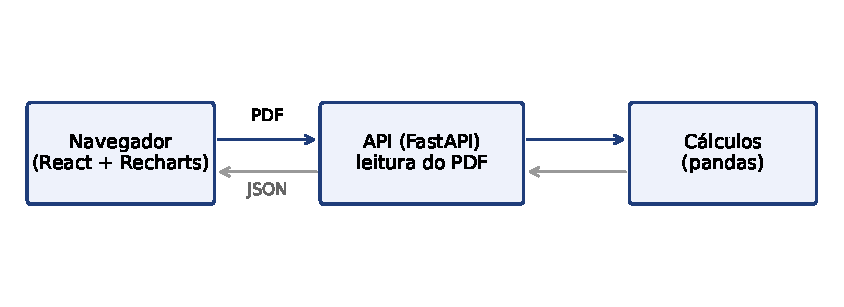
\includegraphics[width=0.9\linewidth]{imagens/arquitetura.pdf}
  \caption{Arquitetura do Cursor}
  \label{fig:arquitetura}
\end{figure}

\subsection{Leitura do histórico}

A leitura do PDF segue três passos:

\begin{enumerate}
  \item a biblioteca pdfplumber \cite{pdfplumber} extrai o texto de cada página do arquivo;
  \item uma expressão regular reconhece as linhas que descrevem uma disciplina, com período, código, carga horária, conceito e situação. Como o nome da disciplina fica na linha de cima, as linhas em maiúsculas logo acima são juntadas para formar o nome;
  \item o pandas padroniza os nomes, remove repetições e ordena as disciplinas por período.
\end{enumerate}

Os valores que o próprio SIGAA imprime, como o CRG e a tabela de carga horária, também são lidos e servem de ponto de partida para os cálculos, afim de que o painel mostre os mesmos números do documento oficial.

\subsection{Privacidade}

O histórico contém dados pessoais do aluno. Por isso, o arquivo é lido na memória e descartado ao fim da requisição, e a ferramenta não usa banco de dados. Para simular o próximo semestre, o navegador reenvia os dados que já recebeu, em vez de o servidor guardá-los. Além disso, a API só aceita arquivos que começam com a assinatura de um PDF, com até 5 MB e 20 páginas.

\section{Resultados} \label{sec:resultados}

Esta seção apresenta a ferramenta em funcionamento, usando um histórico fictício criado para os testes, e descreve como a sua qualidade foi verificada.

\subsection{Interface}

Ao abrir o Cursor, o aluno encontra uma página inicial com visual de jornal, que explica o que a ferramenta faz e onde enviar o PDF (Figura~\ref{fig:tela}). Quem não tem um histórico em mãos pode clicar em ``Ver com um histórico fictício'' e explorar a ferramenta com dados de exemplo.

\begin{figure}[h]
  \centering
  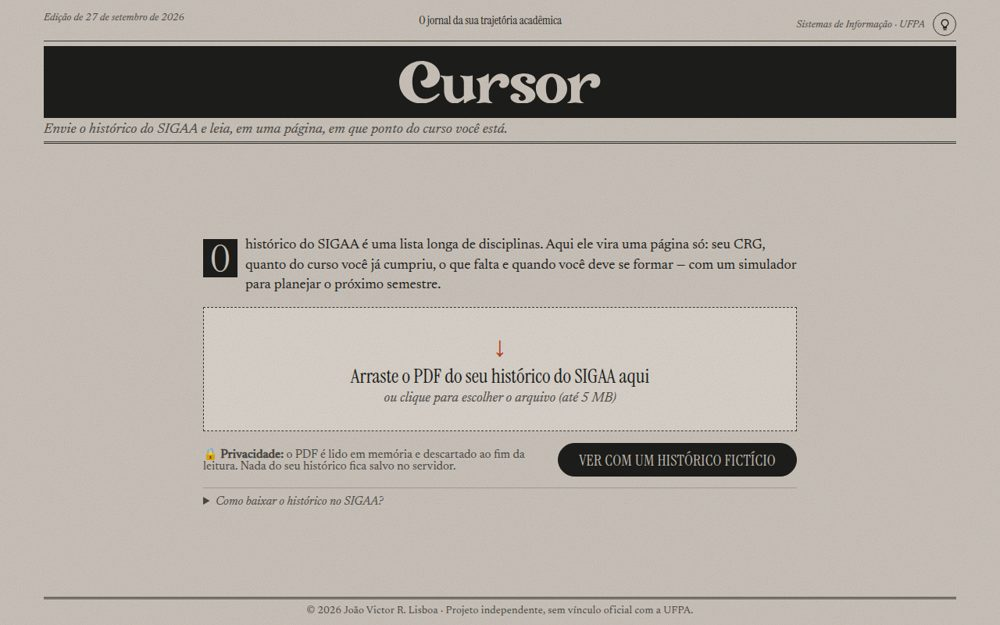
\includegraphics[width=0.9\linewidth]{imagens/tela-inicial.jpg}
  \caption{Tela inicial do Cursor}
  \label{fig:tela}
\end{figure}

Depois de ler o arquivo, o painel mostra o CR de cada período em um gráfico de linha, como mostra a imagem 3. No histórico fictício, o aluno teve uma queda no segundo período e se recuperou nos seguintes, algo que o CRG sozinho não deixaria perceber. O painel também separa os semestre intensivos, cursados nas férias, dos regulares.

\begin{figure}[h]
  \centering
  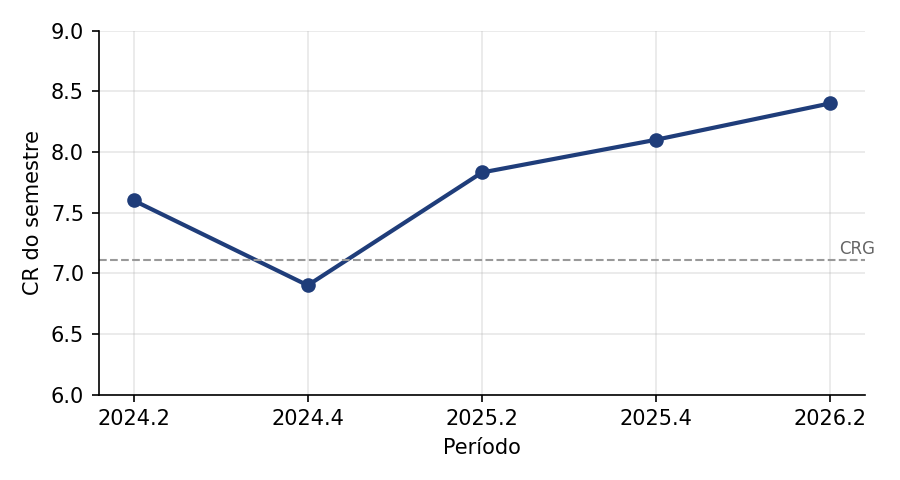
\includegraphics[width=0.8\linewidth]{imagens/cr-semestres.png}
  \caption{Tela inicial do Cursor}
  \label{fig:tela}
\end{figure}

\subsection{Simulador do próximo semestre}

O simulador permite que o aluno escolha as disciplinas que pretende cursar e o conceito que espera obter em cada uma. A partir disso, o Cursor recalcula o CRG, o percentual do curso concluído e a previsão de formatura, mostrando o antes e o depois lado a lado. O cálculo parte do CRG oficial e acrescenta apenas as disciplinas simuladas, para que o resultado continue coerente com o historico do aluno.

\subsection{Testes}

A qualidade da ferramenta foi verificada com testes automatizados escritos com pytest \cite{pytest}. Eles cobrem a leitura do PDF, os cálculos e a API, incluindo casos de erro como arquivo inválido, arquivo grande demais e dados dados fora do formato esperado. Os testes rodam automaticamente a cada alteração enviada ao repositório, e uma nova versão do site só é publicada se todos passarem.

\section{Considerações Finais} \label{sec:conclusao}

O Cursor mostrou que é possível transformar um documento extenso em um painel claro, sem guardar dados do aluno.Em seguida, pretende-se ampliar a leitura para históricos de outros cursos, cujos modelos de PDF variam, e permitir comparar duas simulações diferentes de próximo semestre.

\bibliographystyle{sbc}
\bibliography{sbc-template}

\end{document}
